\documentclass[12pt]{report}

% import and apply GIRS "formatting.sty" file
\usepackage{import}
\usepackage{formatting}

% source-code listings (used in Appendix A)
\usepackage{listings}
\lstset{
    basicstyle=\ttfamily\footnotesize,
    breaklines=true,
    showstringspaces=false,
    numbers=left,
    numberstyle=\tiny,
    frame=single,
    captionpos=b,
    language=Python,
    inputencoding=utf8,
    extendedchars=true,
    literate=
        {—}{{\textemdash}}1
        {–}{{\textendash}}1
        {…}{{\ldots}}1
        {'}{{\textquoteright}}1
        {'}{{\textquoteleft}}1
        {"}{{\textquotedblleft}}1
        {"}{{\textquotedblright}}1
}

% figures live in ./figures/
\graphicspath{{figures/}}

% [H] float placement -- keeps each screenshot pinned exactly where it
% is placed in the source instead of drifting to a later page (the
% default [h!] gives up and floats forward when a figure is nearly a
% full page tall, which is the case for most screenshots here).
\usepackage{float}

% load hyperref last to minimize conflicts
\usepackage{xcolor}
\usepackage[linktocpage=true]{hyperref}
\hypersetup{colorlinks=true, linkcolor=blue, citecolor=blue}

%-------------------------------------------------------
\begin{document}

%-------------------------------------------------------
\frontmatter
%-------------------------------------------------------
% TITLE PAGE
% Assignment requirement: "Start with identifying yourself
% and provide a title for your report."
%-------------------------------------------------------

\begin{center}
\vspace*{60pt}

{\fontsize{18pt}{0pt} \textbf{%
    Assignment 3
    % TODO: title of the report
    }}
\vspace*{100pt}

{\fontsize{14pt}{0pt} \textbf{%
    Fernando Melo Filho
    % TODO: your full name
    }}
\vspace*{2pt}

% {\fontsize{14pt}{0pt} \sf{%
%     <Student ID>
%     % TODO: student ID number
%     }}
% \vspace*{2pt}

{\fontsize{14pt}{0pt} \sf{%
    fmelofilho2950@floridapoly.edu
    % TODO: institutional email
    }}
\vspace*{24pt}

{\fontsize{14pt}{0pt} \textbf{%
    CAP 5410 --- Computer Vision
    }}

\vspace*{2pt}
{\fontsize{14pt}{0pt} \sf{%
    Assignment 3
    }}

\vspace*{24pt}
{\fontsize{14pt}{0pt} \sf{%
    Instructor: Dr. Muhammad Abid
    % TODO: instructor name
    }}

\vspace*{60pt}
{\fontsize{12pt}{0pt} \sf{%
    Convolutional Neural Networks for MNIST Digit Classification
    % TODO: e.g. subject of the lab
    }}

\vspace{\stretch{8}}

{\fontsize{12pt}{0pt} \sf{
    Department of Computer Science \\
    Florida Polytechnic University, Florida, USA }} \\
\vspace*{\fill}

{\fontsize{12pt}{0pt} \sf{
    October 2026
    % TODO: submission month and year
    }}

\end{center}
\thispagestyle{empty}

% \phantomsection
% \include{Abstract}
% \phantomsection
% \include{Acknowledgments}

\phantomsection
\insertTOC
\setcounter{tocdepth}{2}

\phantomsection
\insertLOF

\phantomsection
\insertLOT

%-------------------------------------------------------
\mainmatter
\chapter{Introduction}
\label{ch:intro}

%-------------------------------------------------------

In Assignment 2 I applied box, Sobel and Gaussian filters, whose kernels
are fixed by formula. A convolutional neural network (CNN) uses the same
sliding-window operation, but it learns the kernel values from labeled
examples \citep{goodfellow2016}. In this assignment I implemented a small CNN in
PyTorch \citep{paszke2019}, trained it to recognize handwritten digits
from the MNIST dataset, followed how it learns batch by batch and epoch
by epoch, and ran a controlled experiment on the learning rate.

%%%%%%%%%%%%%%%%%%%%%%%%%%%%%%%%%%%%%%%%%%%%%%%%%%%%%
\section{Objectives}
\label{sec:objectives}
%%%%%%%%%%%%%%%%%%%%%%%%%%%%%%%%%%%%%%%%%%%%%%%%%%%%%

The assignment has five tasks:

\begin{enumerate}
  \item Implement the CNN in PyTorch and document every layer, its
        input/output dimensions, its trainable parameters and the
        training configuration.
  \item Train the baseline for 10 epochs and plot the training loss,
        accuracy and F1-score batch by batch during the first epoch.
  \item Plot training and validation loss, accuracy and F1-score over
        the 10 epochs and discuss convergence and over/underfitting.
  \item Change one hyperparameter (I chose the learning rate), train the
        alternatives under the same conditions, and pick the best
        configuration using validation data only.
  \item Evaluate the chosen model once on the reserved test set and
        document how to reproduce every result.
\end{enumerate}


%%%%%%%%%%%%%%%%%%%%%%%%%%%%%%%%%%%%%%%%%%%%%%%%%%%%%
\section{Background}
\label{sec:background}
%%%%%%%%%%%%%%%%%%%%%%%%%%%%%%%%%%%%%%%%%%%%%%%%%%%%%

\subsection{Training}

The network outputs 10 scores (logits), one per digit. The cross-entropy
loss turns them into probabilities with softmax and penalizes a low
probability on the correct class:
\begin{equation}
  \mathcal{L} = -\frac{1}{N} \sum_{n=1}^{N} \log
  \frac{e^{z_{n,y_n}}}{\sum_{c=0}^{9} e^{z_{n,c}}}
  \label{eq:ce}
\end{equation}
where $z_{n,c}$ is the score of image $n$ for class $c$ and $y_n$ is its
true label. Training repeats four steps for every mini-batch: forward
pass, loss, back-propagation of the gradients, and a parameter update
\citep{abidl08}. With stochastic gradient descent (SGD) with momentum
$\mu$, the update for parameters $\theta$ with learning rate $\eta$ is
\begin{equation}
  v \leftarrow \mu v + \nabla_\theta \mathcal{L}, \qquad
  \theta \leftarrow \theta - \eta\, v
  \label{eq:sgd}
\end{equation}
The learning rate controls the step size, which is why it is the factor
I study in Task 4.

\subsection{Evaluation Metrics}

Accuracy is the fraction of correctly classified images. For each class
$c$, precision $P_c$ is the fraction of images predicted as $c$ that
really are $c$, and recall $R_c$ is the fraction of images of class $c$
that the model finds. The F1-score is their harmonic mean,
$F1_c = 2 P_c R_c / (P_c + R_c)$. Throughout this report I use
\emph{macro} averages: the metric is computed for each digit separately
and then averaged with equal weight over the set of digits $C$,
\begin{equation}
  \text{macro-F1} = \frac{1}{|C|} \sum_{c \in C} F1_c
  \label{eq:macrof1}
\end{equation}
so a digit the model handles badly lowers the score even if it is rare.
On the full training, validation and test sets, $C$ is all 10 digits.
All three are computed with scikit-learn \citep{pedregosa2011}
(\texttt{average="macro"}).


%%%%%%%%%%%%%%%%%%%%%%%%%%%%%%%%%%%%%%%%%%%%%%%%%%%%%
\section{Report Organization}
\label{sec:organization}
%%%%%%%%%%%%%%%%%%%%%%%%%%%%%%%%%%%%%%%%%%%%%%%%%%%%%

Chapter \ref{ch:setup} describes the dataset, the data split and the
seeding shared by all tasks. Each of the five tasks then has its own
chapter:

\begin{itemize}
  \item Chapter \ref{ch:task1}: Task 1, CNN implementation and model
        documentation;
  \item Chapter \ref{ch:task2}: Task 2, first-epoch batch-level learning
        analysis;
  \item Chapter \ref{ch:task3}: Task 3, ten-epoch training and validation
        analysis;
  \item Chapter \ref{ch:task4}: Task 4, controlled learning-rate
        experiment;
  \item Chapter \ref{ch:task5}: Task 5, independent testing and
        reproducibility.
\end{itemize}

Chapter \ref{ch:conclusion} summarizes the results and their
limitations, and Appendix \ref{app:source} lists the complete source
code.
   % Introduction
\chapter{Dataset and Experimental Setup}
\label{ch:setup}

%-------------------------------------------------------

The setup below applies to all five tasks. The code is split into five
Python files.
\texttt{dataloader.py} downloads MNIST and builds the data split,
\texttt{model.py} defines the CNN, \texttt{train.py} contains the
training and evaluation loops, and \texttt{plots.py} draws every figure.
\texttt{main.py} runs all five tasks in order and writes a log of the
program output to \texttt{results/output\_log.txt}. I started from the
``CNN for MNIST'' example in the lecture notes \citep{abidl08}, which is
based on the PyTorch tutorials \citep{pytorchtutorial}. I adapted it to
the $28 \times 28$ MNIST images and added the validation split, the
metrics and the experiment.


%%%%%%%%%%%%%%%%%%%%%%%%%%%%%%%%%%%%%%%%%%%%%%%%%%%%%
\section{Dataset and Data Split}
\label{sec:data}
%%%%%%%%%%%%%%%%%%%%%%%%%%%%%%%%%%%%%%%%%%%%%%%%%%%%%

MNIST \citep{lecun1998,mnistkaggle} contains $28 \times 28$ grayscale
images of the handwritten digits 0--9: 60,000 for training and 10,000 for
testing. I load it with \texttt{torchvision.datasets.MNIST}, which
provides the same files as the Kaggle version. The 60,000 training images
are split once into 48,000 for training (80\%) and 12,000 for validation
(20\%) using a random permutation drawn from a generator seeded with 42
(Listing \ref{lst:split}). Every experiment calls the same function with
the same seed, so all of them use the exact same split. The 10,000 test
images are not used for anything until Task 5.

\lstinputlisting[language=Python, firstline=18, lastline=33,
    firstnumber=auto,
    caption={Fixed 80/20 split and normalization statistics (\texttt{dataloader.py}).},
    label={lst:split}]{../dataloader.py}

\textbf{Preprocessing.} Each image goes through two transforms:
\texttt{ToTensor}, which turns the 0--255 pixel values into a
$1 \times 28 \times 28$ float tensor in $[0, 1]$, and \texttt{Normalize},
which subtracts the mean and divides by the standard deviation. I
computed the mean (0.1307) and standard deviation (0.3082) from the
48,000 training images only, so the validation and test images do not
influence the preprocessing. No data augmentation is used. Normalized
inputs are centered around zero, which keeps the first layer's outputs
in a reasonable range at the start of training.


%%%%%%%%%%%%%%%%%%%%%%%%%%%%%%%%%%%%%%%%%%%%%%%%%%%%%
\section{Random Seed and Identical Starting Conditions}
\label{sec:seed}
%%%%%%%%%%%%%%%%%%%%%%%%%%%%%%%%%%%%%%%%%%%%%%%%%%%%%

All experiments use the seed 42. \texttt{set\_seed} (Listing
\ref{lst:seed}) seeds Python, NumPy and PyTorch and turns on PyTorch's
deterministic algorithms. It is called before the network is created, so
every configuration starts from the same initial weights. The training
loader shuffles with its own generator, also seeded with 42, so all runs
see the batches in the same order. Data loading uses
\texttt{num\_workers=0}, which keeps everything in one process.

\lstinputlisting[language=Python, firstline=24, lastline=29,
    firstnumber=auto,
    caption={Seeding every random number generator (\texttt{train.py}).},
    label={lst:seed}]{../train.py}
   % Dataset and experimental setup (shared by all tasks)
\chapter{Task 1 --- CNN Implementation and Model Documentation}
\label{ch:task1}

%-------------------------------------------------------

Task 1 asks for the CNN implementation in PyTorch, the purpose and
input/output dimensions of each layer, a table of trainable parameters
with an explanation of how they were counted, and the training
configuration with a short justification. Section \ref{sec:model} covers
the layers, Section \ref{sec:params} the parameters, Section
\ref{sec:config} the configuration, and Section \ref{sec:loop} the
training loop and how the metrics are calculated.


%%%%%%%%%%%%%%%%%%%%%%%%%%%%%%%%%%%%%%%%%%%%%%%%%%%%%
\section{Architecture and Layer Dimensions}
\label{sec:model}
%%%%%%%%%%%%%%%%%%%%%%%%%%%%%%%%%%%%%%%%%%%%%%%%%%%%%

The network follows the LeNet-5 design \citep{lecun1998}: two
convolutional layers, each followed by ReLU and $2 \times 2$ max pooling,
and then three fully connected layers (Listing \ref{lst:model}). This
meets the minimum requirement of two convolutional layers, one pooling
layer and one fully connected layer.

\lstinputlisting[language=Python, firstline=7, lastline=34,
    firstnumber=auto,
    caption={The CNN (\texttt{model.py}).},
    label={lst:model}]{../model.py}

The purpose of each layer, for one input image, is:

\begin{itemize}
  \item \textbf{conv1} ($1 \times 28 \times 28 \rightarrow 6 \times 28 \times 28$):
        six $5 \times 5$ kernels learn low-level features such as stroke
        edges and line ends, the same kind of features the Sobel filter
        found in Assignment 2. Padding of 2 keeps the size at $28 \times 28$
        (output size $= 28 + 2\cdot2 - 5 + 1 = 28$), so strokes near the
        border are not lost. The lecture example feeds a
        $1 \times 32 \times 32$ image to conv1 without padding
        \citep{abidl08}; padding the $28 \times 28$ MNIST image by 2 pixels
        gives the same $32 \times 32$ input, so every later layer keeps the
        lecture's dimensions.
  \item \textbf{pool1} ($6 \times 28 \times 28 \rightarrow 6 \times 14 \times 14$):
        max pooling halves the resolution and keeps the strongest response
        in every $2 \times 2$ block.
  \item \textbf{conv2} ($6 \times 14 \times 14 \rightarrow 16 \times 10 \times 10$):
        sixteen $5 \times 5$ kernels, each looking at all six maps from
        conv1, combine edges into larger parts of digits such as curves,
        corners and loops. No padding, so $14 - 5 + 1 = 10$.
  \item \textbf{pool2} ($16 \times 10 \times 10 \rightarrow 16 \times 5 \times 5$):
        halves the resolution again.
  \item \textbf{flatten} ($16 \times 5 \times 5 \rightarrow 400$): turns the
        feature maps into one vector for the fully connected layers.
  \item \textbf{fc1} ($400 \rightarrow 120$) and \textbf{fc2}
        ($120 \rightarrow 84$): combine the features from the whole image
        to decide which digit it is.
  \item \textbf{fc3} ($84 \rightarrow 10$): one score per digit. There is
        no softmax here because \texttt{nn.CrossEntropyLoss} applies
        log-softmax internally (Equation \ref{eq:ce}).
\end{itemize}

ReLU is applied after conv1, conv2, fc1 and fc2. ReLU, pooling and
flatten have no parameters.


%%%%%%%%%%%%%%%%%%%%%%%%%%%%%%%%%%%%%%%%%%%%%%%%%%%%%
\section{Trainable Parameters}
\label{sec:params}
%%%%%%%%%%%%%%%%%%%%%%%%%%%%%%%%%%%%%%%%%%%%%%%%%%%%%

A convolutional layer with $C_{in}$ input channels, $C_{out}$ kernels of
size $k \times k$ has $C_{out}(C_{in} k^2 + 1)$ parameters: each kernel
has $C_{in} k^2$ weights plus one bias. A fully connected layer with
$n_{in}$ inputs and $n_{out}$ outputs has $n_{out}(n_{in} + 1)$
parameters. Table \ref{table:params} applies these formulas to every
layer.

\begin{table}[h]
    \centering
    \caption[Trainable parameters per layer.]%
    {Output shape and trainable parameters of every layer, for one input image.}

    \begin{tabular}{c|c|P{2.3in}|r}
        \specialrule{1.5pt}{0pt}{0pt}
        Layer & Output shape & Calculation & Parameters \\
        \hline\hline
        conv1 & $6 \times 28 \times 28$ & $6 \times (1 \cdot 5 \cdot 5 + 1)$ & 156 \\
        \specialrule{0.5pt}{0pt}{0pt}
        pool1 & $6 \times 14 \times 14$ & --- & 0 \\
        \specialrule{0.5pt}{0pt}{0pt}
        conv2 & $16 \times 10 \times 10$ & $16 \times (6 \cdot 5 \cdot 5 + 1)$ & 2,416 \\
        \specialrule{0.5pt}{0pt}{0pt}
        pool2 & $16 \times 5 \times 5$ & --- & 0 \\
        \specialrule{0.5pt}{0pt}{0pt}
        flatten & 400 & --- & 0 \\
        \specialrule{0.5pt}{0pt}{0pt}
        fc1 & 120 & $120 \times (400 + 1)$ & 48,120 \\
        \specialrule{0.5pt}{0pt}{0pt}
        fc2 & 84 & $84 \times (120 + 1)$ & 10,164 \\
        \specialrule{0.5pt}{0pt}{0pt}
        fc3 & 10 & $10 \times (84 + 1)$ & 850 \\
        \hline\hline
        \textbf{Total} & & & \textbf{61,706} \\
        \specialrule{1.5pt}{0pt}{0pt}
    \end{tabular}
    \label{table:params}
\end{table}

To check the hand calculation, \texttt{model.py} also counts the
parameters in code: \texttt{layer\_table} passes a dummy image through
the network with forward hooks to record each layer's output shape, and
sums \texttt{p.numel()} over each layer's tensors. The program prints the
same 61,706 total (Listing \ref{lst:output-params}). Almost 78\% of the
parameters are in fc1, while the two convolutional layers together hold
only about 4\%, because a convolution reuses the same small kernel at
every position of the image.

\begin{lstlisting}[language={}, numbers=none, caption={Program output: layer shapes and parameter counts.}, label={lst:output-params}]
=== Layers (input -> output shape, trainable parameters)
conv1  (1, 28, 28)     -> (6, 28, 28)         156
conv2  (6, 14, 14)     -> (16, 10, 10)       2416
fc1    (400,)          -> (120,)            48120
fc2    (120,)          -> (84,)             10164
fc3    (84,)           -> (10,)               850
total trainable parameters: 61706
\end{lstlisting}


%%%%%%%%%%%%%%%%%%%%%%%%%%%%%%%%%%%%%%%%%%%%%%%%%%%%%
\section{Training Configuration}
\label{sec:config}
%%%%%%%%%%%%%%%%%%%%%%%%%%%%%%%%%%%%%%%%%%%%%%%%%%%%%

\begin{table}[h]
    \centering
    \caption[Baseline training configuration.]%
    {Baseline training configuration.}

    \begin{tabular}{P{1.7in}|P{3.6in}}
        \specialrule{1.5pt}{0pt}{0pt}
        Setting & Value \\
        \hline\hline
        Optimizer & SGD with momentum 0.9 \\
        \specialrule{0.5pt}{0pt}{0pt}
        Learning rate & 0.01 (constant, no scheduler) \\
        \specialrule{0.5pt}{0pt}{0pt}
        Batch size & 64 (750 batches per epoch) \\
        \specialrule{0.5pt}{0pt}{0pt}
        Epochs & 10 \\
        \specialrule{0.5pt}{0pt}{0pt}
        Loss function & Cross-entropy (\texttt{nn.CrossEntropyLoss}) \\
        \specialrule{0.5pt}{0pt}{0pt}
        Weight initialization & PyTorch default, drawn right after seeding \\
        \specialrule{0.5pt}{0pt}{0pt}
        Random seed & 42 (split, initial weights, shuffling) \\
        \specialrule{0.5pt}{0pt}{0pt}
        Preprocessing & ToTensor, then Normalize(mean 0.1307, std 0.3082) \\
        \specialrule{0.5pt}{0pt}{0pt}
        Regularization & None (no dropout, no weight decay) \\
        \specialrule{1.5pt}{0pt}{0pt}
    \end{tabular}
    \label{table:config}
\end{table}

\textbf{Justification.} Cross-entropy is the standard loss for
single-label classification with 10 classes, and it is the loss used in
the lecture's full training example. That example trains with
\texttt{optim.SGD(lr=0.001, momentum=0.9)} and a batch size of 4
\citep{abidl08}. I kept SGD with momentum, which averages recent
gradients and so smooths the noisy mini-batch updates. I used a batch
of 64, which makes each gradient estimate less noisy and an epoch much
faster (750 updates instead of 12,000). With 16 times fewer updates per
epoch, a learning rate of 0.001 would move slowly, so I raised it to
0.01 for the baseline, the value the lecture uses in its
parameter-update example \citep{abidl08}. Task 4 (Chapter
\ref{ch:task4}) tests whether this was a good choice. I left out dropout and weight decay so that the baseline shows
the plain learning behavior of the network, and any overfitting would be
visible in the curves.


%%%%%%%%%%%%%%%%%%%%%%%%%%%%%%%%%%%%%%%%%%%%%%%%%%%%%
\section{Training Loop and Metric Calculation}
\label{sec:loop}
%%%%%%%%%%%%%%%%%%%%%%%%%%%%%%%%%%%%%%%%%%%%%%%%%%%%%

Listing \ref{lst:loop} shows the training loop. For every batch it
clears the old gradients, runs the forward pass, computes the loss,
back-propagates and updates the weights. During the first epoch it also
records, for each batch, the loss, the accuracy and the macro-F1 of that
batch's predictions, plus a cumulative macro-F1 over every image seen so
far in the epoch. These are the values plotted in Task 2 (Chapter
\ref{ch:task2}).

\lstinputlisting[language=Python, firstline=87, lastline=120,
    firstnumber=auto,
    caption={Training loop with first-epoch batch logging (\texttt{train.py}).},
    label={lst:loop}]{../train.py}

At the end of every epoch, \texttt{evaluate} (Listing \ref{lst:evaluate})
runs the model in evaluation mode, without gradients, over the whole
training split and the whole validation split. I measure the training
metrics this way instead of averaging the batch values during the epoch,
because the batch values mix early and late weights from the same epoch.
Re-evaluating both sets with the same end-of-epoch weights makes the
training and validation numbers directly comparable, which matters for
the gap analysis in Task 3 (Chapter \ref{ch:task3}).

Every F1-score in this report is macro-F1 (Equation \ref{eq:macrof1}),
computed by \texttt{macro\_f1} with scikit-learn's
\texttt{f1\_score(average="macro")}: the F1-score of each digit is
computed separately and the values are averaged with equal weight over
the digits that appear in the labels or the predictions. On the full
training, validation and test sets that is always all 10 digits.
Macro-precision and macro-recall for Task 5 are computed the
same way with \texttt{precision\_score} and \texttt{recall\_score}.

\lstinputlisting[language=Python, firstline=32, lastline=57,
    firstnumber=auto,
    caption={Macro-F1 and the evaluation function (\texttt{train.py}).},
    label={lst:evaluate}]{../train.py}
   % Task 1: CNN implementation and model documentation
\chapter{Task 2 --- First-Epoch Batch-Level Learning Analysis}
\label{ch:task2}

%-------------------------------------------------------

Task 2 asks for the training loss, training accuracy and F1-score of the
baseline plotted by batch during the first epoch (2--4 graphs), an
explanation of the learning behavior, and how the F1-score was
calculated. The baseline was trained for the full 10 epochs; this
chapter looks only at epoch 1, and Chapter \ref{ch:task3} covers all 10.

During the first epoch of the baseline (750 batches of 64 images), the
training loop recorded the loss, accuracy and macro-F1 of every batch
(Section \ref{sec:loop}). To keep the plots readable, the faint line
shows only every 5th batch, and the solid line is a 50-batch running
average over all batches. The per-batch macro-F1 is computed on the 64
predictions of that batch alone, with scikit-learn's
\texttt{f1\_score(average="macro")}, averaging over the digits present in
that batch's labels or predictions. A random batch of 64 occasionally
misses a digit entirely (8 of the 750 batches in this epoch), and that
digit is left out of the average instead of being counted as an F1 of
0. Since a batch has only about six images of each digit, one mistake
changes a class's F1 by a lot, so
Figure \ref{fig:epoch1-f1} also shows a cumulative macro-F1 computed over
every image seen so far in the epoch.

\begin{figure}[H]
    \centering
    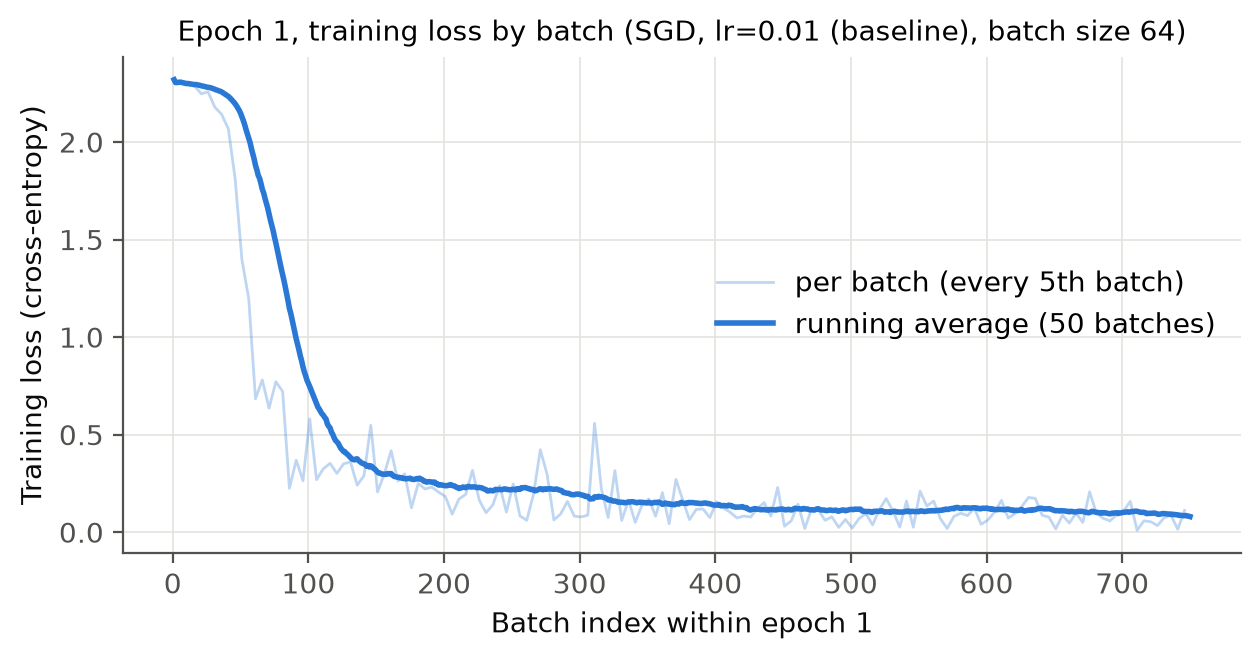
\includegraphics[width = 0.88\textwidth]{epoch1_loss.png}
    \caption[Epoch 1: training loss by batch.]%
    {Baseline (SGD, $\eta = 0.01$, batch size 64): training cross-entropy
    loss during the first epoch.}
    \label{fig:epoch1-loss}
\end{figure}

\begin{figure}[H]
    \centering
    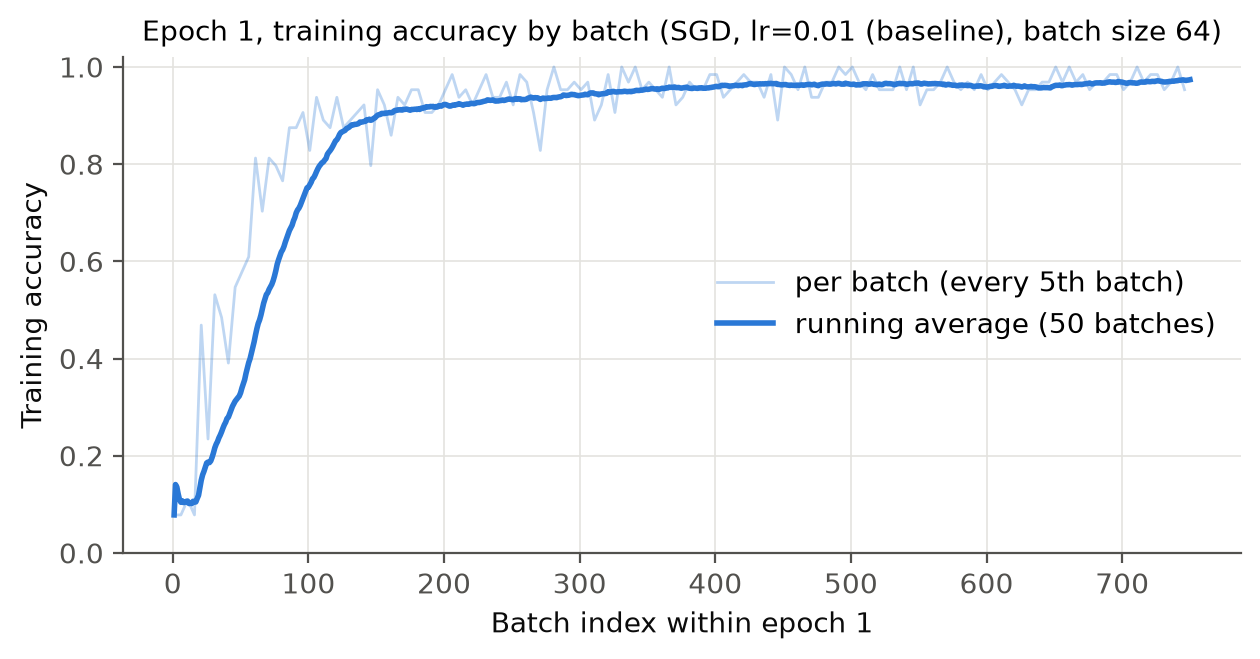
\includegraphics[width = 0.88\textwidth]{epoch1_accuracy.png}
    \caption[Epoch 1: training accuracy by batch.]%
    {Baseline: training accuracy of each batch during the first epoch.}
    \label{fig:epoch1-acc}
\end{figure}

\begin{figure}[H]
    \centering
    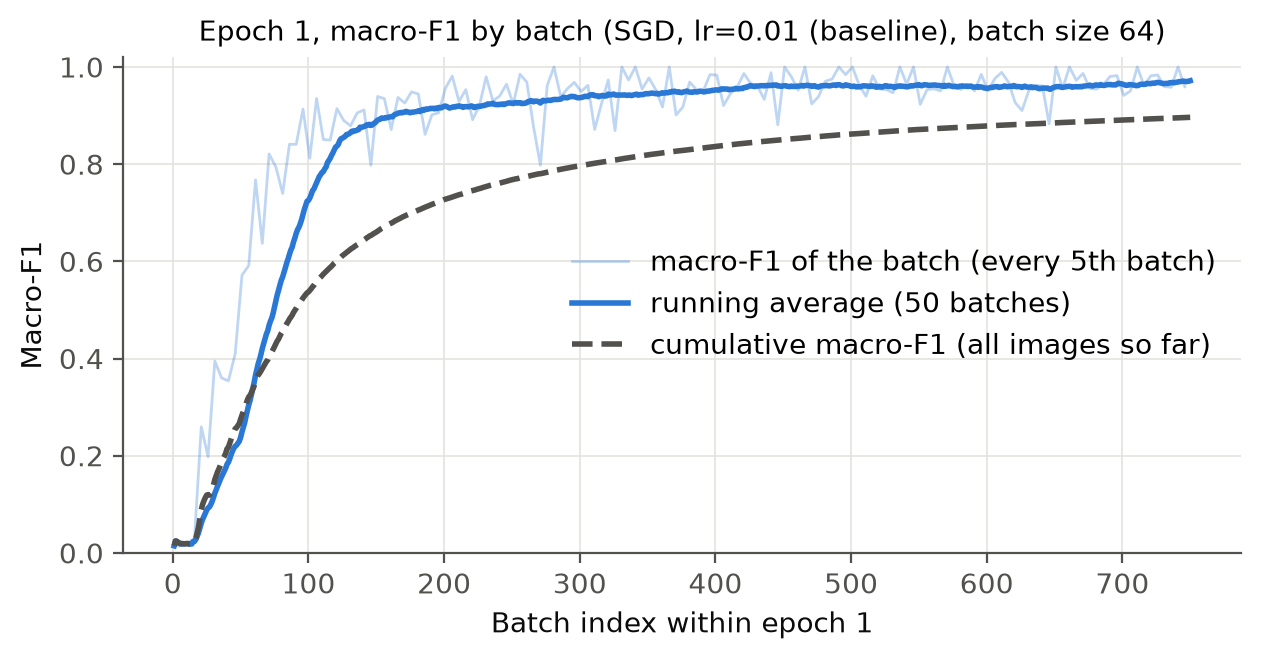
\includegraphics[width = 0.88\textwidth]{epoch1_f1.png}
    \caption[Epoch 1: macro-F1 by batch.]%
    {Baseline: per-batch macro-F1, its running average, and the
    cumulative macro-F1 over all images seen so far in the first epoch.}
    \label{fig:epoch1-f1}
\end{figure}

\textbf{Observation.} The first batch has a loss of 2.32 and an accuracy
of 7.8\%. This is what an untrained network should give: with random
weights, all 10 classes get about the same probability, so the loss is
close to $\ln 10 = 2.30$ and accuracy is close to the 10\% chance level.
The epoch then goes through three phases:

\begin{enumerate}
  \item Slow start (batches 1--40). The loss only goes from 2.32 to
        2.04. The gradients are small at first, and momentum needs a few
        steps to build up speed.
  \item Fast learning (batches 40--150). The loss falls quickly: the
        50-batch average is 2.15 at batch 50, 0.76 at batch 100 and 0.24
        at batch 200. Accuracy and macro-F1 rise together, and the
        running accuracy passes 90\% at batch 151. Most of the epoch's
        improvement happens in these hundred or so batches.
  \item Refinement (batches 150--750). Progress slows down and the
        curves flatten. By the end of the epoch, the running loss is 0.08
        and the running accuracy is 97.4\%.
\end{enumerate}

The per-batch curves stay noisy until the end (in the last 100 batches,
batch accuracy still varies between 92\% and 100\%) because each batch
is a different random sample of 64 images. Accuracy and macro-F1 follow
almost the same path: MNIST classes are nearly balanced, so no digit is
being ignored and the two metrics agree. The cumulative macro-F1 ends at
0.896, well below the late-batch values of about 0.97, because it still
includes the predictions from the start of the epoch when the network was
guessing.
   % Task 2: first-epoch batch-level analysis
\chapter{Task 3 --- Ten-Epoch Training and Validation Analysis}
\label{ch:task3}

%-------------------------------------------------------

Task 3 asks for the training and validation loss and accuracy of the
baseline over the 10 epochs, the epoch-level macro-F1, and a discussion
of convergence, the training--validation gap and any over- or
underfitting. Only epoch-level summaries are used here.

At the end of every epoch, the training split (48,000 images) and the
validation split (12,000 images) were evaluated with the same weights in
evaluation mode (Section \ref{sec:loop}). Table \ref{table:epochs} lists
the values, and Figures \ref{fig:epochs-loss}--\ref{fig:epochs-f1} plot
them.

\begin{table}[h]
    \centering
    \caption[Baseline epoch-level metrics.]%
    {Baseline (SGD, $\eta = 0.01$, batch size 64): epoch-level loss,
    accuracy and macro-F1 on the training and validation splits.}

    \begin{tabular}{c|c|c|c|c|c|c}
        \specialrule{1.5pt}{0pt}{0pt}
        Epoch & Train loss & Train acc. & Train F1 & Val. loss & Val. acc. & Val. F1 \\
        \hline\hline
        1  & 0.0903 & 97.23\% & 0.9722 & 0.1084 & 96.75\% & 0.9673 \\
        2  & 0.0575 & 98.14\% & 0.9812 & 0.0724 & 97.78\% & 0.9776 \\
        3  & 0.0431 & 98.61\% & 0.9859 & 0.0693 & 97.83\% & 0.9781 \\
        4  & 0.0413 & 98.67\% & 0.9866 & 0.0643 & 98.27\% & 0.9826 \\
        5  & 0.0261 & 99.16\% & 0.9915 & 0.0557 & 98.31\% & 0.9829 \\
        6  & 0.0227 & 99.28\% & 0.9927 & 0.0574 & 98.29\% & 0.9827 \\
        7  & 0.0136 & 99.58\% & 0.9958 & \textbf{0.0425} & \textbf{98.77\%} & \textbf{0.9876} \\
        8  & 0.0131 & 99.59\% & 0.9959 & 0.0473 & 98.63\% & 0.9862 \\
        9  & 0.0248 & 99.11\% & 0.9909 & 0.0558 & 98.54\% & 0.9853 \\
        10 & 0.0129 & 99.56\% & 0.9956 & 0.0473 & 98.68\% & 0.9867 \\
        \specialrule{1.5pt}{0pt}{0pt}
    \end{tabular}
    \label{table:epochs}
\end{table}

\begin{figure}[H]
    \centering
    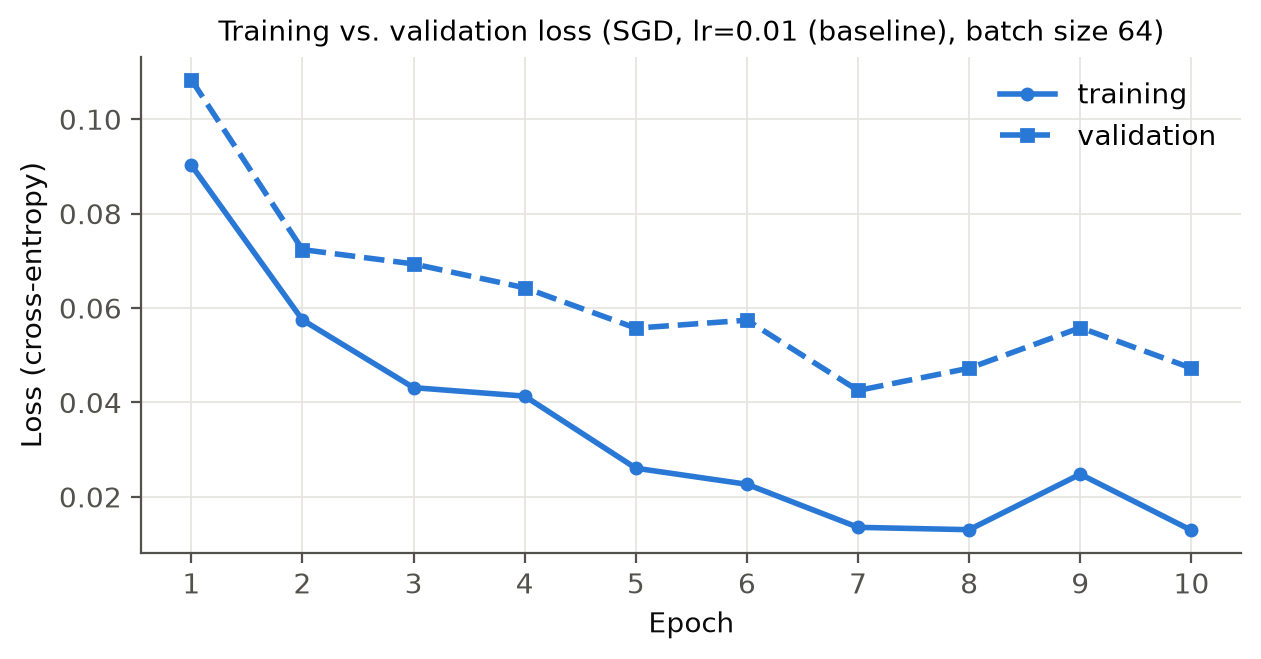
\includegraphics[width = 0.88\textwidth]{epochs_loss.png}
    \caption[Training and validation loss over 10 epochs.]%
    {Baseline: training and validation cross-entropy loss per epoch.}
    \label{fig:epochs-loss}
\end{figure}

\begin{figure}[H]
    \centering
    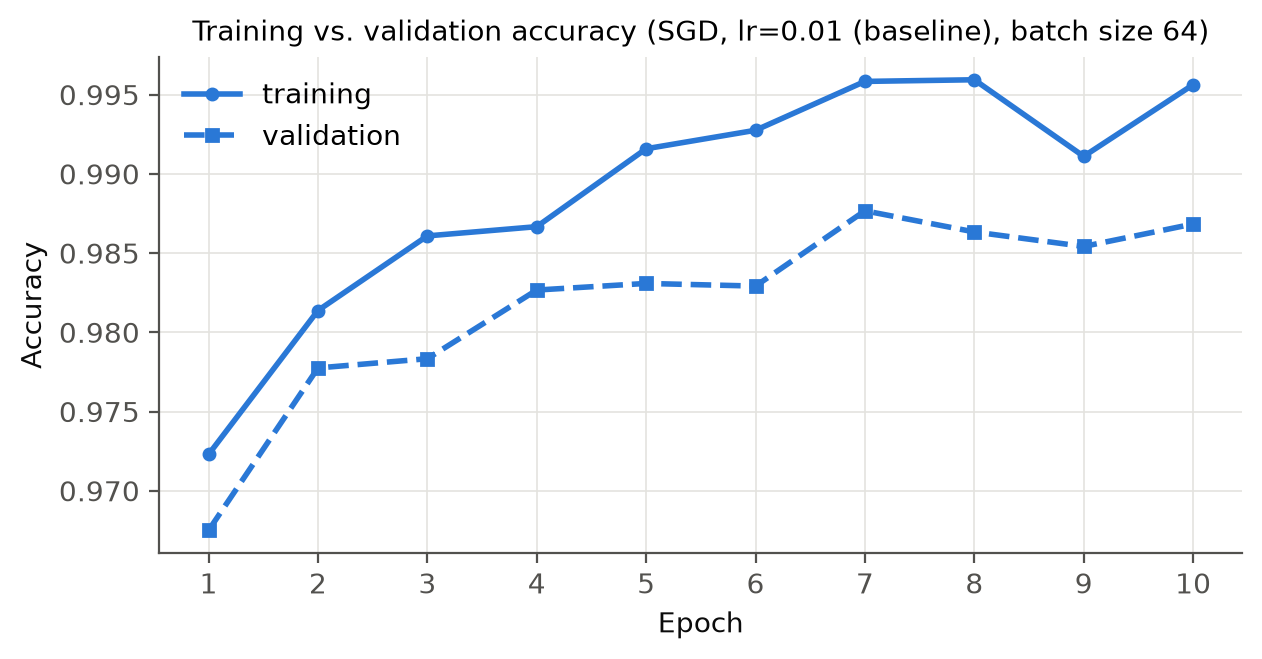
\includegraphics[width = 0.88\textwidth]{epochs_accuracy.png}
    \caption[Training and validation accuracy over 10 epochs.]%
    {Baseline: training and validation accuracy per epoch.}
    \label{fig:epochs-acc}
\end{figure}

\begin{figure}[H]
    \centering
    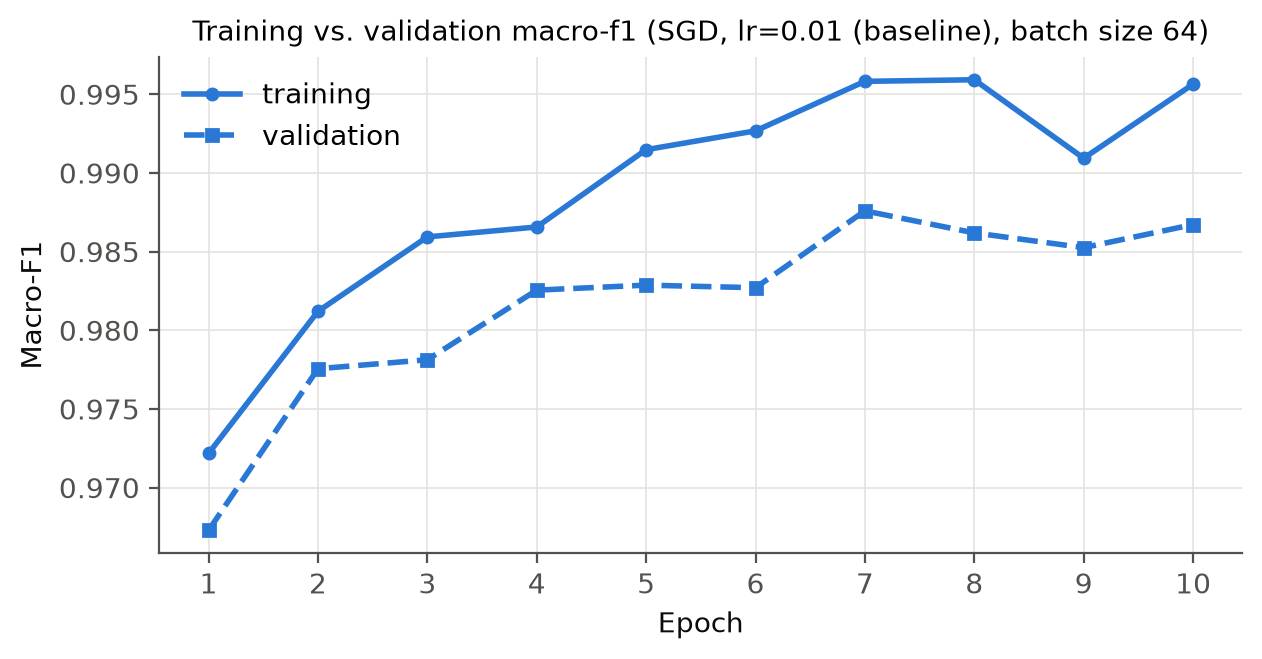
\includegraphics[width = 0.88\textwidth]{epochs_f1.png}
    \caption[Training and validation macro-F1 over 10 epochs.]%
    {Baseline: training and validation macro-F1 per epoch.}
    \label{fig:epochs-f1}
\end{figure}

\textbf{Convergence.} Most of the learning happens in the first epoch:
after it, validation accuracy is already 96.75\%. The next epochs add
smaller gains, and validation accuracy stays between 98.27\% and
98.77\% from epoch 4 on. The best validation epoch is epoch 7 (loss
0.0425, accuracy 98.77\%). After that the validation curves stop
improving and move up and down within about 0.25 percentage points, so
the model has converged by about epoch 7. Epoch 9 shows a small
bump: training loss rises from 0.0131 to 0.0248 and validation loss from
0.0473 to 0.0558, and both recover in epoch 10. With a constant
learning rate and momentum, a few unlucky batches can push the weights
slightly away from a good point. The training and validation curves
move together here, so I read it as optimization noise. Overfitting
would show up as validation loss rising while training loss falls.

\textbf{Training--validation gap.} Training is better than validation at
every epoch, and the gap grows over time. In accuracy it goes from 0.48
percentage points at epoch 1 to 0.88 points at epoch 10; in loss, the
training loss at epoch 10 (0.0129) is less than a third of the
validation loss (0.0473). Macro-F1 follows accuracy almost exactly on
both sets (differences of at most 0.0002), so the errors are spread
across the digits.

\textbf{Overfitting and underfitting.} There is no underfitting: the
network reaches 99.6\% training accuracy, so it has enough capacity for
this task. There is \emph{mild} overfitting after epoch 7: the training
loss keeps going down while the validation loss stops improving (0.0425
at epoch 7, then 0.047--0.056), so the extra epochs mostly fit the
training images more tightly. The effect is small, though. Validation
accuracy does not drop in any meaningful way (98.68\% at epoch 10
against 98.77\% at its best), and the final model still generalizes
well. Dropout or weight decay could reduce the gap further, and early
stopping around epoch 7 would be another option.
   % Task 3: ten-epoch training and validation analysis
\chapter{Task 4 --- Controlled Learning-Rate Experiment}
\label{ch:task4}

%-------------------------------------------------------

Task 4 asks me to choose one factor, compare the baseline with at least
one alternative under otherwise fixed settings, train each for 10
epochs, compare their curves, and explain which configuration I would
select and why. Section \ref{sec:experiment-design} describes the
setup and Section \ref{sec:task4} the results and the selection.

%%%%%%%%%%%%%%%%%%%%%%%%%%%%%%%%%%%%%%%%%%%%%%%%%%%%%
\section{Experiment Design}
\label{sec:experiment-design}
%%%%%%%%%%%%%%%%%%%%%%%%%%%%%%%%%%%%%%%%%%%%%%%%%%%%%

The factor I chose to study is the learning rate. Besides the baseline
($\eta = 0.01$), I trained two alternatives, one ten times smaller
($\eta = 0.001$) and one ten times larger ($\eta = 0.1$). Everything else
is identical to Table \ref{table:config}: same optimizer and momentum,
same batch size, same split, same seed, same initial weights and same
batch order. The three configurations are listed at the top of
\texttt{main.py} (Listing \ref{lst:configs}).

\lstinputlisting[language=Python, firstline=30, lastline=39,
    firstnumber=auto,
    caption={The three configurations (\texttt{main.py}).},
    label={lst:configs}]{../main.py}

\textbf{Selection rule.} The rule was fixed before looking at any
results: the configuration with the highest validation accuracy after
epoch 10 is selected, with lower validation loss as the tie-breaker. The
test set is only loaded after this choice is made, and only once.


%%%%%%%%%%%%%%%%%%%%%%%%%%%%%%%%%%%%%%%%%%%%%%%%%%%%%
\section{Results and Selection}
\label{sec:task4}
%%%%%%%%%%%%%%%%%%%%%%%%%%%%%%%%%%%%%%%%%%%%%%%%%%%%%

Figure \ref{fig:compare} shows the
training and validation curves side by side, Figure
\ref{fig:compare-epoch1} compares the first epoch, Figure
\ref{fig:compare-val} zooms in on validation accuracy, and Table
\ref{table:compare} summarizes the results.

\begin{figure}[H]
    \centering
    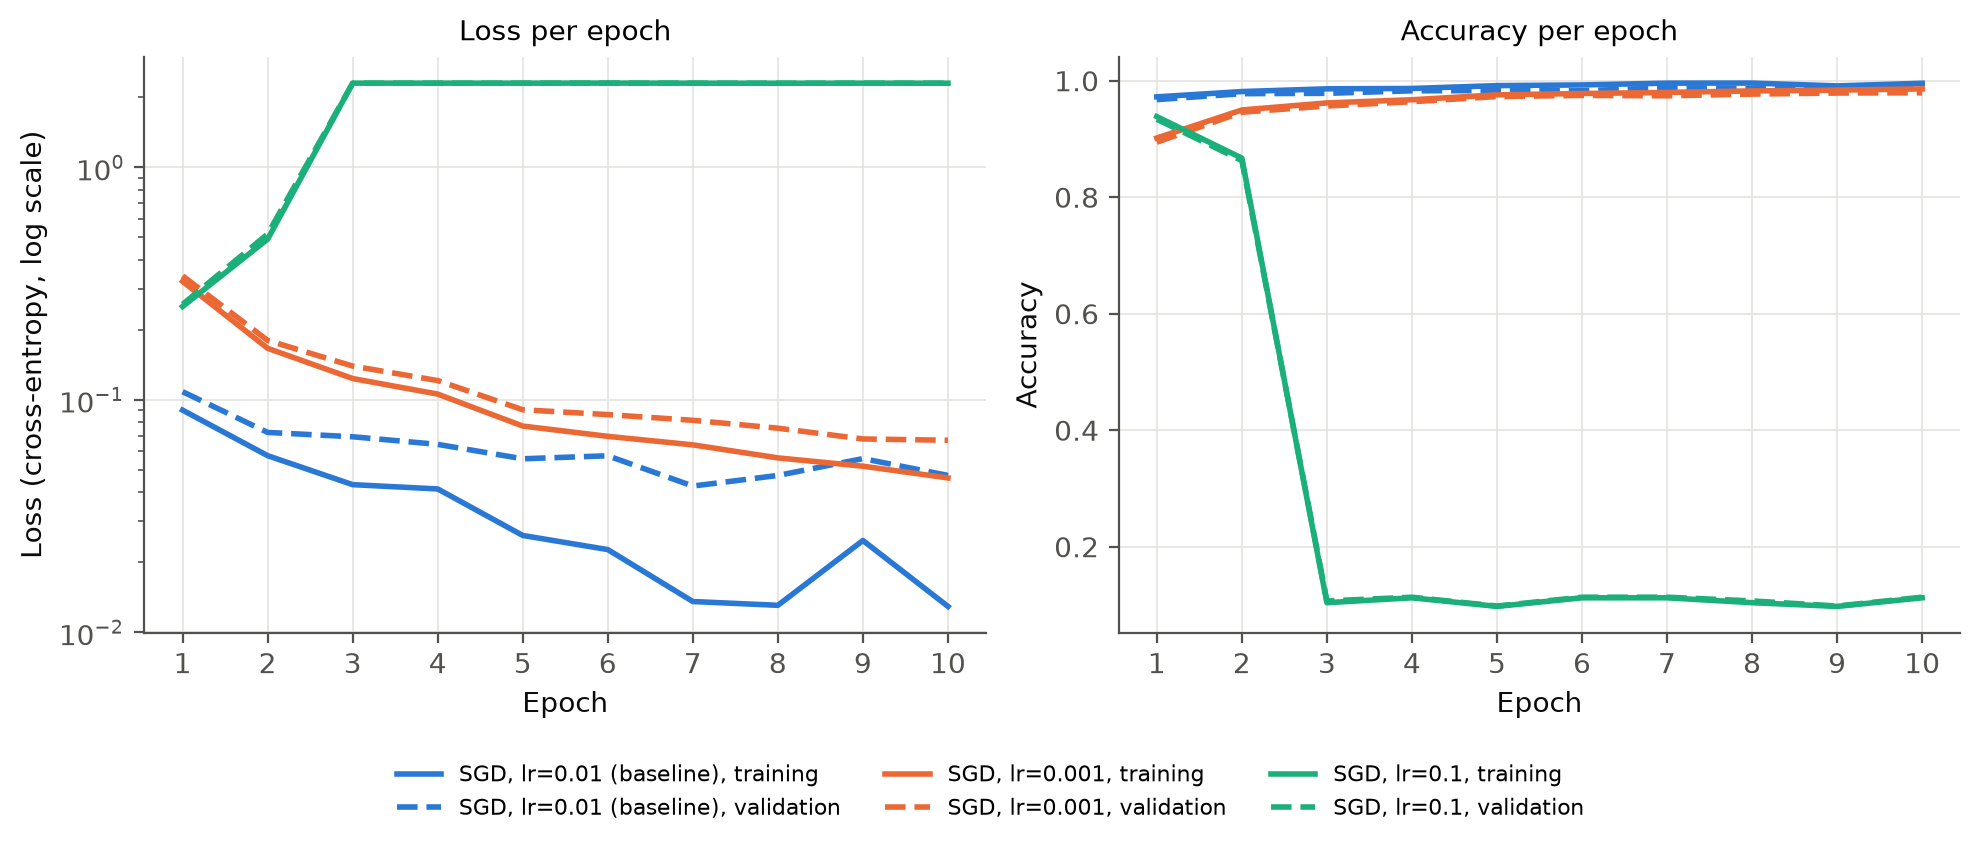
\includegraphics[width = \textwidth]{compare_curves.png}
    \caption[Learning-rate comparison: loss and accuracy curves.]%
    {Training (solid) and validation (dashed) loss and accuracy per epoch
    for the three learning rates (SGD, momentum 0.9, batch size 64). The
    loss axis is logarithmic.}
    \label{fig:compare}
\end{figure}

\begin{figure}[H]
    \centering
    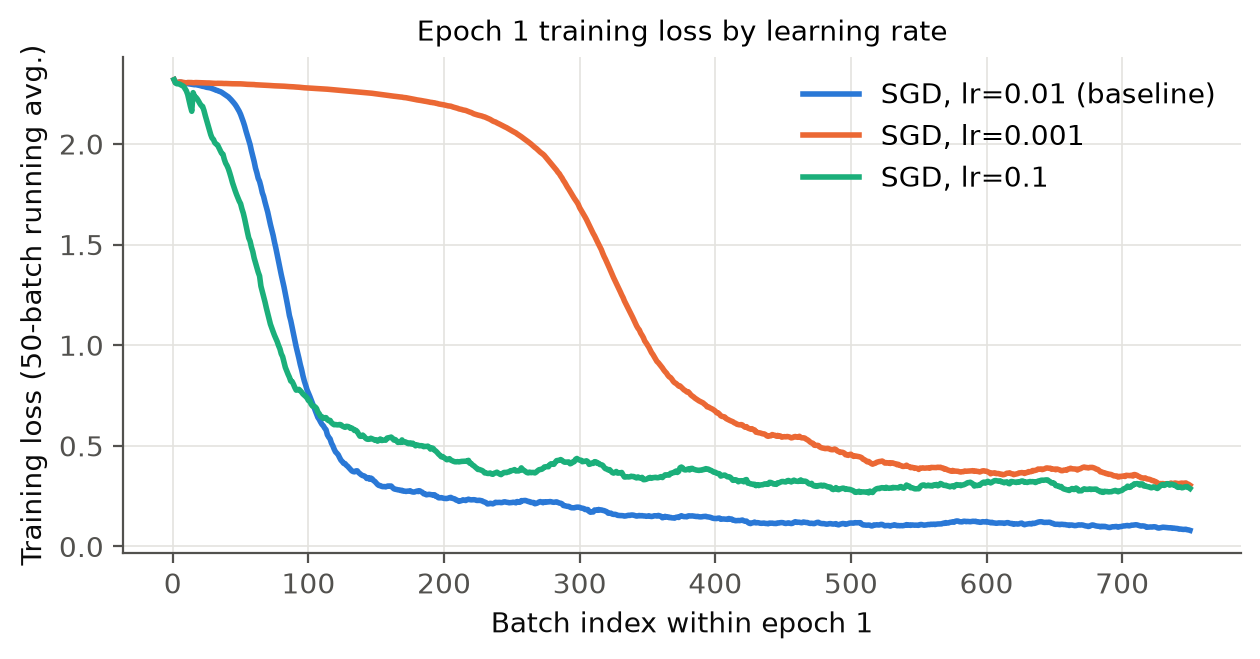
\includegraphics[width = 0.88\textwidth]{compare_epoch1_loss.png}
    \caption[Learning-rate comparison: first-epoch loss.]%
    {Training loss (50-batch running average) during the first epoch for
    the three learning rates.}
    \label{fig:compare-epoch1}
\end{figure}

\begin{figure}[H]
    \centering
    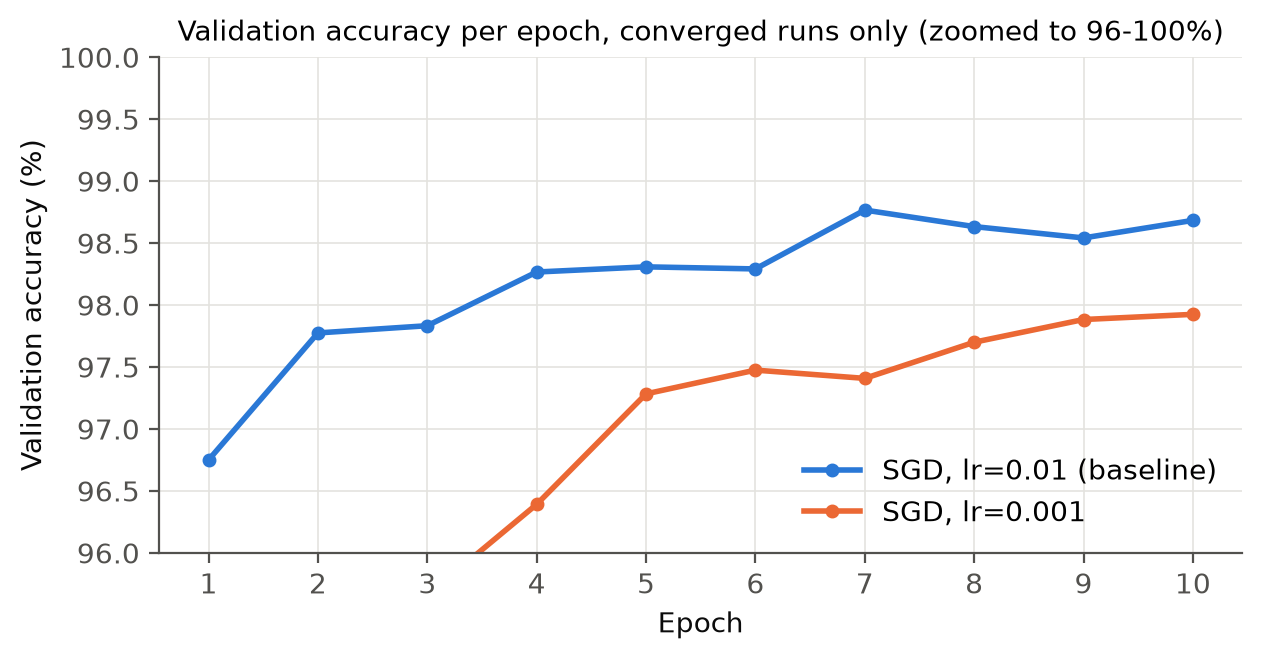
\includegraphics[width = 0.88\textwidth]{compare_val_acc.png}
    \caption[Learning-rate comparison: validation accuracy (zoom).]%
    {Validation accuracy per epoch for $\eta = 0.01$ and $\eta = 0.001$,
    zoomed to 96--100\%. The $\eta = 0.1$ run is left out because it stays
    near 11\% after epoch 3.}
    \label{fig:compare-val}
\end{figure}

\begin{table}[h]
    \centering
    \caption[Learning-rate comparison summary.]%
    {Learning-rate comparison. Final values are after epoch 10; the gap
    is training accuracy minus validation accuracy at epoch 10.}

    \begin{tabular}{l|c|c|c}
        \specialrule{1.5pt}{0pt}{0pt}
        & $\eta = 0.001$ & $\eta = 0.01$ (baseline) & $\eta = 0.1$ \\
        \hline\hline
        Val.\ accuracy after epoch 1 & 89.44\% & 96.75\% & 93.38\% \\
        \specialrule{0.5pt}{0pt}{0pt}
        Batch where running acc.\ passes 90\% & 714 & 151 & 228 \\
        \specialrule{0.5pt}{0pt}{0pt}
        Final training accuracy & 98.60\% & 99.56\% & 11.22\% \\
        \specialrule{0.5pt}{0pt}{0pt}
        Final validation accuracy & 97.92\% & \textbf{98.68\%} & 11.33\% \\
        \specialrule{0.5pt}{0pt}{0pt}
        Final validation macro-F1 & 0.9790 & \textbf{0.9867} & 0.0203 \\
        \specialrule{0.5pt}{0pt}{0pt}
        Final validation loss & 0.0670 & \textbf{0.0473} & 2.3030 \\
        \specialrule{0.5pt}{0pt}{0pt}
        Best validation accuracy (epoch) & 97.92\% (10) & 98.77\% (7) & 93.38\% (1) \\
        \specialrule{0.5pt}{0pt}{0pt}
        Train--val.\ accuracy gap & 0.67 pts & 0.88 pts & --- \\
        \specialrule{1.5pt}{0pt}{0pt}
    \end{tabular}
    \label{table:compare}
\end{table}

\textbf{Small learning rate ($\eta = 0.001$): too slow.} With steps ten
times smaller, the network stays on the initial plateau much longer. In
the first epoch the loss is still 2.19 after 200 batches, and the running
accuracy passes 90\% only at batch 714, almost five times later than the
baseline (Figure \ref{fig:compare-epoch1}). After one epoch it has 89.4\%
validation accuracy, against 96.8\% for the baseline. It keeps
improving steadily and never shows instability, but after 10 epochs it
reaches only 97.92\%, about where the baseline was after epoch 3. Its
validation loss is still going down at epoch 10, so this run has not
converged yet: it is slightly \emph{underfitting} within the 10-epoch
budget. Its train--validation gap is the smallest (0.67 points), but
only because it has not fit the training data as tightly yet.

\textbf{Large learning rate ($\eta = 0.1$): fast, then unstable.} At first
the large steps help: in Figure \ref{fig:compare-epoch1} its loss falls
earlier than the baseline's. But the curve is noisier, with a loss spike
to 3.55 at batch 15, and in the second half of the epoch its loss stays
higher (0.30 on average, against 0.11 for the baseline), because the steps are too big
to settle into a good minimum. After epoch 1 its validation accuracy is
93.4\%. In epoch 2 it gets worse (86.3\%), and in epoch 3 training
collapses. From then on the loss stays at 2.303, which is exactly
$\ln 10$, and accuracy stays at about 11\%: the network has collapsed to
predicting the same digit for every image, which is why its validation
macro-F1 is only 0.0203. Training and validation accuracy are equally
bad, which points to a failure of the optimization itself.

\textbf{Selection.} Following the rule set in Section
\ref{sec:experiment-design}, the selected configuration is the
\textbf{baseline, $\eta = 0.01$}. It has the highest final validation
accuracy (98.68\%), the highest validation macro-F1 (0.9867) and the
lowest validation loss (0.0473). It also converges much faster than
$\eta = 0.001$ and is stable, while $\eta = 0.1$ diverges. Its
generalization gap (0.88 points) is a little larger than that of
$\eta = 0.001$, but its validation accuracy is still 0.76 points higher.
With more epochs $\eta = 0.001$ might catch up. Within the 10 epochs
required here, 0.01 is the better choice.
   % Task 4: learning-rate experiment
\chapter{Task 5 --- Independent Testing and Reproducibility}
\label{ch:task5}

%-------------------------------------------------------

Task 5 asks for a single evaluation of the selected configuration on the
reserved MNIST test set, reporting accuracy, macro-precision,
macro-recall and macro-F1, together with the random seed, the library
versions, the execution environment and instructions to reproduce the
experiments. These are covered in Sections \ref{sec:task5},
\ref{sec:environment} and \ref{sec:repro}.

%%%%%%%%%%%%%%%%%%%%%%%%%%%%%%%%%%%%%%%%%%%%%%%%%%%%%
\section{Test-Set Evaluation}
\label{sec:task5}
%%%%%%%%%%%%%%%%%%%%%%%%%%%%%%%%%%%%%%%%%%%%%%%%%%%%%

Only after the configuration was selected did \texttt{main.py} load the
10,000 test images, evaluating the saved epoch-10 weights of the baseline
once. Listing \ref{lst:test-output} shows the program output and Table
\ref{table:test} the metrics.

\begin{lstlisting}[language={}, numbers=none, caption={Program output: model selection and the single test evaluation.}, label={lst:test-output}]
=== Validation summary after epoch 10
lr_0.01   val acc 0.9868  val F1 0.9867  val loss 0.0473  best val acc 0.9877 (epoch 7)
lr_0.001  val acc 0.9792  val F1 0.9790  val loss 0.0670  best val acc 0.9792 (epoch 10)
lr_0.1    val acc 0.1133  val F1 0.0203  val loss 2.3030  best val acc 0.9338 (epoch 1)
selected configuration: lr_0.01

=== TEST (lr_0.01, evaluated once)
test_loss        0.0402
test_acc         0.9884
macro_precision  0.9882
macro_recall     0.9885
macro_f1         0.9883
\end{lstlisting}

\begin{table}[h]
    \centering
    \caption[Test-set results.]%
    {Test-set results of the selected model (SGD, $\eta = 0.01$, batch
    size 64, weights after epoch 10, seed 42).}

    \begin{tabular}{P{2.4in}|c}
        \specialrule{1.5pt}{0pt}{0pt}
        Metric & Test set (10,000 images) \\
        \hline\hline
        Accuracy & 98.84\% \\
        \specialrule{0.5pt}{0pt}{0pt}
        Macro-precision & 0.9882 \\
        \specialrule{0.5pt}{0pt}{0pt}
        Macro-recall & 0.9885 \\
        \specialrule{0.5pt}{0pt}{0pt}
        Macro-F1 & 0.9883 \\
        \specialrule{0.5pt}{0pt}{0pt}
        Cross-entropy loss & 0.0402 \\
        \specialrule{1.5pt}{0pt}{0pt}
    \end{tabular}
    \label{table:test}
\end{table}

\textbf{Observation.} The model classifies 9,884 of the 10,000 test
images correctly, so it makes 116 errors. The test accuracy (98.84\%)
is close to the validation accuracy (98.68\%), and slightly higher. The
validation set was therefore a good estimate of performance on unseen
data, and selecting on it did not overfit to the validation images.
Macro-precision, macro-recall and macro-F1 are all within 0.0003 of the
accuracy, so no digit is much worse than the others.


%%%%%%%%%%%%%%%%%%%%%%%%%%%%%%%%%%%%%%%%%%%%%%%%%%%%%
\section{Execution Environment and Library Versions}
\label{sec:environment}
%%%%%%%%%%%%%%%%%%%%%%%%%%%%%%%%%%%%%%%%%%%%%%%%%%%%%

\begin{table}[h]
    \centering
    \caption[Software and hardware environment.]%
    {Software and hardware environment used for every experiment.}

    \begin{tabular}{P{1.6in}|P{1.4in}|P{2.4in}}
        \specialrule{1.5pt}{0pt}{0pt}
        Component & Version & Purpose \\
        \hline\hline
        Python & 3.13.5 & Programming language \\
        \specialrule{0.5pt}{0pt}{0pt}
        PyTorch & 2.14.1 (CPU build) & Tensors, layers, autograd, optimizer \citep{paszke2019} \\
        \specialrule{0.5pt}{0pt}{0pt}
        torchvision & 0.29.1 & MNIST download and transforms \\
        \specialrule{0.5pt}{0pt}{0pt}
        scikit-learn & 1.9.1 & Precision, recall and F1 \citep{pedregosa2011} \\
        \specialrule{0.5pt}{0pt}{0pt}
        NumPy / Matplotlib & 2.5.4 / 3.11.2 & Arrays and figures \citep{hunter2007} \\
        \specialrule{0.5pt}{0pt}{0pt}
        Operating system & Windows 11 Home & 64-bit \\
        \specialrule{0.5pt}{0pt}{0pt}
        Hardware & Intel Core i7-13700F, 16~GB RAM & All training on the CPU (16 threads); no GPU used \\
        \specialrule{1.5pt}{0pt}{0pt}
    \end{tabular}
    \label{table:environment}
\end{table}

The computer has an NVIDIA RTX 4060 Ti, but I installed the CPU build of
PyTorch on purpose. The network is small enough to train on the CPU in a
few minutes, and on the CPU \texttt{torch.use\_deterministic\_algorithms(True)}
makes every run give the same numbers, which is harder to guarantee with
GPU kernels.


%%%%%%%%%%%%%%%%%%%%%%%%%%%%%%%%%%%%%%%%%%%%%%%%%%%%%
\section{Instructions to Reproduce the Experiments}
\label{sec:repro}
%%%%%%%%%%%%%%%%%%%%%%%%%%%%%%%%%%%%%%%%%%%%%%%%%%%%%

All results in this report were produced by the code in Appendix
\ref{app:source} on the machine in Table \ref{table:environment}. To
reproduce them:

\begin{enumerate}
  \item Install Python 3.13 and create a virtual environment in the
        project folder:
\begin{lstlisting}[language={}, numbers=none]
python -m venv env
env\Scripts\activate          (Windows)
source env/bin/activate       (Linux / macOS)
\end{lstlisting}
  \item Install the pinned dependencies (CPU build of PyTorch):
\begin{lstlisting}[language={}, numbers=none]
pip install -r requirements.txt
\end{lstlisting}
  \item Run all experiments. MNIST is downloaded to \texttt{./data} on
        the first run (internet needed once):
\begin{lstlisting}[language={}, numbers=none]
python main.py
\end{lstlisting}
        This trains the three configurations (about 10 minutes in total on
        the CPU above), selects one using the validation set, evaluates
        it once on the test set, and writes:
        \begin{itemize}
          \item \texttt{results/output\_log.txt}: the full program output;
          \item \texttt{results/<config>/history.json} and
                \texttt{model.pt}: metrics and final weights per
                configuration;
          \item \texttt{results/test\_metrics.json}: the test metrics;
          \item \texttt{report/figures/*.png}: every figure in this report.
        \end{itemize}
  \item To redo only the selection, the test evaluation and the figures
        from saved results, run \texttt{python main.py --skip-train}.
\end{enumerate}

\textbf{Random seed.} Seed 42 is used for the train/validation split,
the initial weights and the shuffling order (Section \ref{sec:seed}).
Training runs on the CPU with
\texttt{torch.use\_deterministic\_algorithms(True)} and
\texttt{num\_workers=0}, so running \texttt{main.py} again on the same
software versions gives the same numbers. I checked this by training all
three configurations a second time: every epoch-level loss, accuracy and
F1-score, and the final weights, matched the first run exactly.
Different PyTorch versions or a GPU may change the last digits because
of floating-point differences.
   % Task 5: independent testing and reproducibility
\chapter{Conclusion}
\label{ch:conclusion}

%-------------------------------------------------------

In this assignment I implemented a LeNet-style CNN in PyTorch with two
convolutional layers, two pooling layers and three fully connected layers
(61,706 parameters), and trained it on a fixed 48,000/12,000 split of
MNIST. During the first epoch, the model went from chance level to over
97\% accuracy. Over 10 epochs it converged by about epoch 7, with mild
overfitting after that. In the learning-rate experiment, 0.001 was too
slow to converge in 10 epochs and 0.1 collapsed in epoch 3, so the
baseline of 0.01 was selected on the validation set. Evaluated once on
the 10,000 test images, it reached 98.84\% accuracy, 0.9882
macro-precision, 0.9885 macro-recall and 0.9883 macro-F1.

\textbf{Limitations.} Each configuration was trained with a single seed,
so differences of a few tenths of a percent between runs should be read
with care. Only three learning rates, a factor of 10 apart, were tested,
and the reported model uses the weights from the end of epoch 10, even
though epoch 7 had a slightly better validation score.
   % Discussion and conclusion

%-------------------------------------------------------
\backmatter
\bibliographystyle{ascelike}
\bibliography{references}

\begin{appendices}
\appendix
\addtocontents{toc}{\protect\setcounter{tocdepth}{0}}
\addtocontents{toc}{\protect\renewcommand{%
    \protect\chapterprefix}{%
    \protect\hspace*{-0.5in}APPENDIX\protect\hspace*{0.6in}}}%

%%%%%%%%%%%%%%%%%%%%%%%%%%%%%%%%%%%%%%%%%%%%%%%%%%%%%
%%% APPENDIX CONTENTS
%%%%%%%%%%%%%%%%%%%%%%%%%%%%%%%%%%%%%%%%%%%%%%%%%%%%%

\chapter{Source Code}
\label{app:source}

The complete source files are listed below; they are the same files
submitted alongside this report.

\section{dataloader.py}
\lstinputlisting[language=Python, caption={MNIST loading and data split (\texttt{dataloader.py}).}, label={lst:dataloader}]{../dataloader.py}

\section{model.py}
\lstinputlisting[language=Python, caption={CNN and parameter table (\texttt{model.py}).}, label={lst:modelfull}]{../model.py}

\section{train.py}
\lstinputlisting[language=Python, caption={Training, evaluation and testing (\texttt{train.py}).}, label={lst:trainfull}]{../train.py}

\section{main.py}
\lstinputlisting[language=Python, caption={Experiment driver (\texttt{main.py}).}, label={lst:mainfull}]{../main.py}

\section{plots.py}
\lstinputlisting[language=Python, caption={Figures (\texttt{plots.py}).}, label={lst:plotsfull}]{../plots.py}
   % Full source code
\end{appendices}


\end{document}
%-------------------------------------------------------
